\section{Intrinsic vs. Extrinsic Evaluation of Czech Sentence Embeddings}
\label{extrinsic}

In the previous sections, we focused on \emph{intrinsic evaluation} of sentence embeddings, examining how their internal geometric structure reflects semantic relations. Using the \costra dataset, we showed that current models struggle to capture language phenomena such as gradual stylistic change, temporal shifts, or logical opposition, and instead rely heavily on surface-level similarity.

However, as discussed in \Cref{prehistory}, this thesis is primarily concerned with machine translation evaluation (MTE). In this setting, embeddings are not evaluated in isolation, but as components of evaluation metrics. Their usefulness is therefore better assessed through \emph{extrinsic evaluation}, particularly in MTE and quality estimation (QE), where embeddings are used to compare translations, references, and source sentences.

However, intrinsic and extrinsic evaluation differ substantially in cost. Extrinsic evaluation typically requires training or fine-tuning models (e.g., within the \comet framework) for each candidate embedding, while intrinsic evaluation can be performed directly using simple similarity computations. This makes intrinsic evaluation much cheaper and easier to reproduce.

This leads to a natural question: can intrinsic evaluation serve as a proxy for downstream performance? Semantic Textual Similarity (STS) is closely related to MTE/QE, as both tasks assess whether two sentences convey the same meaning despite surface differences. If intrinsic benchmarks correlated well with extrinsic performance, they could be used as a quick proxy for selecting promising embedding models. However, prior work (\Cref{extrinsic:rw}) suggests that STS is not a reliable predictor of downstream effectiveness. Whether this also holds for machine translation evaluation remains unclear.

This question is particularly relevant given the growing number of available embedding models. Multilingual encoders such as \labse and \xlmr provide strong cross-lingual representations, while language-specific models aim to better capture properties of individual languages. For morphologically rich languages such as Czech, it is not obvious which approach is more suitable for MT evaluation. A reliable intrinsic proxy would make it possible to narrow down candidates before expensive MTE/QE training.

% This raises a question: \emph{to what extent do intrinsic and extrinsic evaluation agree in the context of machine translation evaluation?} If intrinsic benchmarks reliably predict downstream performance, they could serve as an efficient model selection tool. If not, they capture only a limited subset of the properties required for MT evaluation.

In this section\footnote{This section is based on \cite{barancikova-bojar-2025-intrinsic}. I was responsible for the experimental design, implementation, and evaluation. Ond\v{r}ej Bojar contributed through consultations and co-authoring the resulting publication.}, we compare intrinsic and extrinsic evaluation for Czech sentence embeddings. We evaluate Czech-specific and multilingual models using (i) intrinsic benchmarks (\costra, STS) and (ii) extrinsic evaluation based on \comet fine-tuning for MTE and QE. Our goal is to determine not only which embeddings perform the best, but also whether intrinsic properties translate into downstream effectiveness in this setting.

\pagebreak

\begin{mdframed}[
    linecolor=gray,
    linewidth=2pt,
    roundcorner=5,
    backgroundcolor=gray!5
]
\noindent
In particular, we address the following research questions:
\begin{itemize}
    \item Can intrinsic evaluation serve as a reliable predictor of embedding performance in MTE/QE?
    \item Do Czech-specific encoders outperform multilingual models in evaluation of Czech translations?
    \item Does model size matter after fine-tuning in MTE/QE?
\end{itemize}
\end{mdframed}

\subsection{Related Work}
\label{extrinsic:rw}
Several studies have already questioned the suitability of STS for embedding selection. For example, \cite{reimers-etal-2016-task}, \cite{pitfalls2019}, and \cite{zhelezniak-etal-2019-correlation} argue that, while STS can capture certain semantic similarities, it does not reliably predict how effective sentence representations will be for downstream tasks. These works show that STS tasks often encourage surface-level heuristics or oversimplified semantic similarity patterns that may not generalize to more complex applications like entailment or paraphrasing detection. 

To address these limitations, new intrinsic evaluation methods such as EvalRank \citep{wang-etal-2022-just} and SentBench \citep{xiaoming-etal-2023-sentbench} have been proposed, both of which exhibit a~stronger correlation with extrinsic evaluation measures. These benchmarks evaluate sentence representations through information retrieval, sentence ordering, and probing tasks, offering a more holistic view of embedding quality that aligns better with actual downstream task performance. %TODO: jen pro anglictinu?

It is important to note that these previous experiments did not specifically focus on machine translation evaluation, which seems to be very close to~STS, in the sense that they both compare pairs of sentences and evaluate their semantic similarity. \cite{cifka-bojar-2018-bleu} report a negative correlation between the translation quality of the Transformer models measured by \bleu and the semantic properties (assessed using STS) of the sentence embeddings derived from the Transformer model. In contrast, \cite{libovicky-probing} demonstrate a strong positive correlation between STS performance and translation quality for both Transformer and RNN-based models. %These conflicting results underscore the complexity of linking intrinsic evaluation metrics to performance in machine translation tasks.

While this work focuses on evaluating MT metrics themselves, our work instead examines sentence embeddings as building blocks of modern neural evaluation metrics. In this setting, we ask a complementary question: whether intrinsic evaluation of embeddings (e.g., STS or \costra) can predict their effectiveness when used within MT evaluation frameworks such as \comet.

\cite{freitag-etal-2022-results} have advocated for the use of semantic-aware metrics such as \bertscore \citep{bertscore:2020} and \comet \citep{rei-etal-2020-comet} in MT evaluation, showing that these outperform \bleu in correlating with human judgments. These models incorporate contextual embeddings and often exhibit closer alignment with human-perceived meaning, bringing MT evaluation closer to the goals of intrinsic semantic understanding.

\subsection{Models}
For our experiments, we used several state-of-the-art sentence embedding models. We include all Czech embedding models described in \Cref{examined-embeddings}: \czert, \fernet, \robeczech, \retromae, and \simcse. 

For multilingual encoders, we selected three widely used models with different training objectives. The multilingual \mepet encoder is based on contrastive pre-training on targeting semantic similarity and retrieval tasks \citep{wang2024multilingual}, and is therefore well suited to intrinsic evaluation based on similarity judgments. The \labse model is trained using translation ranking objectives to align sentence representations across languages \citep{feng-etal-2022-language}. We also include \xlmr, a general-purpose multilingual encoder trained with masked language modeling \citep{xlm-r}, which is not specifically optimized for sentence-level similarity but shows strong performance in downstream applications.

This selection allows us to compare models with different training signals and to examine how these differences affect both intrinsic and extrinsic evaluation.  As control models, we again employ \randombert and \random. \Cref{tab:model_comparison_detailed} provides a brief overview of their architectures.

\subsection{Intrinsic Evaluation}
We first evaluate the embeddings on several semantic benchmarks to examine how accurately they capture various semantic properties of sentences.

\paragraph{Costra}
\noindent
As the first dataset for intrinsic evaluation, we used the \costra-- dataset \citep{costra11}, which we described in detail in the previous section. As established in \Cref{costra:results}, current sentence encoders struggle to move beyond surface-level heuristics. For the purposes of this comparative study, we focus on the \costraminus aggregate score, which measures the models' ability to capture scalable semantic relations (\textbf{Time}, \textbf{Style}, \textbf{Generalization}, and \textbf{Opposition}) while excluding the ``impossible'' \textbf{Basic} and \textbf{Modality} categories.

The results, summarized in the last column of \Cref{tab:costra_results}, show that the distilled \simcse model achieves the strongest intrinsic grasp of these relations (0.72), however, the differences among the trained models are not significant. In fact, the best models performed only marginally better than the \randombert baseline, suggesting limited success in capturing the phenomena tested in the \costra dataset, such as linearity of time or generalization. 

\paragraph{Semantic textual similarity}
\noindent
\begin{table}[tb]
    \centering
 \begin{tabular}{lccccc}
\toprule
\textbf{Embeddings} & \textbf{CNA} & \textbf{SVOB\_IMG} & \textbf{SVOB\_HL}  & \textbf{mean}\\
\midrule
\simcse     & 88.56 & \textbf{90.73} & \textbf{84.22} & \textbf{87.83} \\
\mepet      & \textbf{89.25} & 90.13 & 82.77 & 87.38 \\
\labse     & 85.54 & 85.58 & 77.62 & 82.91 \\
\retromae   & 82.96 & 79.10 & 63.63 & 76.30 \\
\czert      & 84.10 & 77.04 & 63.24 & 74.79 \\
\robeczech  & 76.35 & 71.24 & 60.64 & 69.41\\
\fernet    & 78.22 & 63.59 & 54.56 & 65.46 \\
\randombert    & 65.56 & 63.70 & 52.17 & 60.48 \\
\xlmr      & 68.48 & 51.70 & 45.19 & 55.12 \\
\bottomrule
\end{tabular}
    \caption{Results of intrinsic evaluation on three STS datasets. We used the best performing pooling method and cosine similarity as similarity function.}
    \label{tab:STS}
\end{table}

We evaluate STS on three datasets. The first dataset, CNA, comes from the test set of \citet{sido2021czert} and contains 1,100 sentence pairs together with similarity labels selected from Czech journalistic texts. These labels were collected by averaging nine independent human annotations, providing a high-quality reference for semantic equivalence judgments.

The remaining two datasets, SVOB-IMG and SVOB-HL, were created by \citep{DBLP:conf/tsd/SvobodaB18} as Czech adaptations of the SentEval STS benchmark \citep{senteval}. SVOB-IMG includes 850 sentence pairs derived from image captions, focusing on descriptive and contextually rich sentences. SVOB-HL consists of 525 sentence pairs from news headlines. Both datasets were translated from English into Czech and manually re-annotated for semantic similarity.

We evaluated all models using the automated evaluation tool\footurl{https://github.com/seznam/czech-semantic-embedding-models} provided by \citet{bednavr2024some}. For precomputed sentence embeddings, this tool explores different embedding similarity metrics including cosine similarity, dot product, and Manhattan distance. Additionally, it applies various sentence embeddings pooling strategies and selects the highest average score as the final result. 

Interestingly, the STS results (\Cref{tab:STS}) are consistent with the findings from \costra, with \simcse being the overall best performing model, followed by \mepet, \labse and \retromae.
\xlmr, despite being a large multilingual encoder, performs worst, even below \randombert. This is in line with \cite{litschko:2022}, who show that multilingual encoders such as mBERT and \xlmr often underperform on sentence-level semantic similarity tasks without task-specific fine-tuning. 

This consistency between STS and \costra results provides additional support for the validity of the \costra benchmark, despite its more challenging and structured evaluation setup.

\subsection{Extrinsic Evaluation --- MTE and QE}
As our extrinsic evaluation, we selected two tasks: machine translation evaluation and quality estimation. These tasks are very similar -- both evaluate the quality of a translation hypothesis, MTE with respect to reference translations, QE as a reference-free evaluation. Both tasks may incorporate the source sentence as additional context. A more detailed discussion of these tasks is provided in~\Cref{rw}.

\subsubsection{Data}
In the following experiments, we use datasets from the Workshop on Machine Translation (WMT), selecting data from English-to-Czech translations. These datasets include English source sentences, Czech hypotheses, Czech reference sentences, and the human translation quality scores collected using the Direct Assessment (DA) method \citep{graham-etal-2013-continuous} and subsequently \texttt{z}-normalized to take individual annotator bias into account by centering and scaling scores of each annotator. For more detail on human evaluation we refer to \Cref{sec:human_evaluation}.

Data from WMT17 to WMT19 \citep{wmt2017, bojar-etal-2018-findings, barrault-etal-2019-findings} were used to train the \comet estimators \citep{rei-etal-2020-comet}. The validation of the models was performed on the WMT20 dataset \citep{barrault-etal-2020-findings}, and the performance of the models was tested using the WMT21 \cite{akhbardeh-etal-2021-findings} and WMT22 \citep{kocmi-etal-2022-findings} datasets.

\subsubsection{MTE Baseline Approach}
\begin{table}[tb]
    \centering
\resizebox{\textwidth}{!}{%
\begin{tabular}{l|ccc|cccc}
 &  \multicolumn{3}{|c|}{\textbf{WMT21 test set}} &  \multicolumn{4}{|c}{\textbf{WMT22 test set}} \\
 \toprule
\textbf{Embeddings} & $\rho_{H,R}$ & $\rho_{H,S}$ & $S_{C}(S,R)$ & $\rho_{H,R}$  & $\rho_{H,S}$ & $S_{C}(S,R)$  & $S_{C}(S_{R},R_{R})$ \\
\midrule
\mepet   & \textbf{0.29} & 0.04 & 0.89 & 0.26 & 0.01 & 0.90 & 0.75 \\
\retromae & 0.26 & -0.10 & 0.76 & \textbf{0.27} & \textbf{0.09} & 0.76 & 0.69 \\
\simcse   & 0.24 & \textbf{0.13} & 0.85 & 0.25 & 0.05 & 0.82 & 0.09 \\
\czert   & 0.20 & -0.03 & 0.63 & 0.18 & -0.06 & 0.62 & 0.52 \\
\xlmr   & 0.17 & -0.08 & 1.00 & 0.05 & -0.10 & 1.00 & 0.99 \\
\robeczech & 0.15 & -0.16 & 0.92 & 0.11 & -0.06 & 0.91 & 0.89 \\
\labse    & 0.11 & 0.03  & 0.89 & 0.19 &  0.06 & 0.88 & 0.31 \\
\fernet  & 0.07 & -0.11 & 0.45 & 0.11 & -0.03 & 0.40 & 0.35 \\
\randombert & 0.06 & -0.16 & 0.99 & 0.03 & -0.20 & 0.98 & 0.98 \\
\bottomrule
\end{tabular}
}
    \caption{Results of the baseline MTE approach -- using sentence embeddings for direct evaluation without fine-tuning. $\rho_{H,R}$ represents Pearson correlation between human quality assessments and the cosine similarity between the translation hypothesis and the reference translation, while $\rho_{H,S}$ shows the correlation between human judgments and the cosine similarity between the hypothesis and the source sentence. $S_{C}(S,R)$ represents cosine similarity between references and sources. The last column represents cosine similarity between randomly shuffled source and reference sentences averaged over 100 runs on WMT22 data.}
    \label{tab:baseline}
\end{table}

Before fine-tuning embedding based metrics for machine translation evaluation and quality estimation, we conducted a preliminary analysis to assess their default ability to evaluate translation quality. Specifically, we examined Pearson's correlation between human judgments and the cosine similarities computed between (i) a hypothesis and a reference translation ($\rho_{H,R}$) and (ii) a hypothesis and a source sentence ($\rho_{H,S}$). We expected high cosine similarity for multilingual models, reflecting their ability to capture cross-lingual semantic relationships, whereas Czech-specific models---lacking such cross-lingual information---were anticipated to have random similarity scores.

Furthermore, we examined the intrinsic quality of the embedding spaces by measuring the cosine similarity between the source and reference embeddings ($S_{C}(S,R)$). We also performed a random shuffling experiment designed to evaluate the discriminative ability of the embeddings.

The results presented in \Cref{tab:baseline} reveal that even without fine-tuning, a slight correlation between human judgments and cosine similarity of hypotheses and references ($\rho_{H,R}$ columns) is observable in certain models---particularly \mepet, \retromae, and \simcse. However, contrary to expectations, this does not hold for source sentences ($\rho_{H,S}$ columns); no relationship was detected between human evaluation scores and the cosine similarity computed between a translated sentence and its source sentence, even among the multilingual models.

The analysis of the embedding space via similarity between source and reference sentences provides further insights $(S_{C}(S,R)$ columns). In line with our hypothesis, \xlmr exhibits a near perfect similarity between the source and reference sentences, which suggest that the \xlmr embedding space may be overly compressed for the Czech language before task-specific training. In this state, the high-dimensional vectors are compressed into such a narrow cone that the model loses the resolution necessary to distinguish between semantic equivalence and random noise, causing even unrelated shuffled pairs to appear identical.

To further investigate this behavior, we repeated the experiment using random shuffle of source and reference sentences; see the last column of \Cref{tab:baseline} (column $S_{C}(S_{R},R_{R})$). The similarity remained perfect for both \xlmr and \randombert even on shuffled pairs, indicating an overly invariant embedding space, where even pairs of semantically unrelated sentences tend to cluster together. This \emph{over-smoothing} reduces the model's capacity to distinguish subtle differences that are essential for evaluating translation quality. In such cases, even bad translations can receive high similarity scores, lowering the correlation with human judgment. This also explains the poor performance of \xlmr in our intrinsic evaluation task, especially in the STS task (\Cref{tab:STS}).
More broadly speaking, it casts doubts on any results based on the direct similarity of \xlmr embedding vectors in the Czech language, given that \xlmr assigns similar vectors to all tested sentence pairs from WMT22.

\subsubsection{Training \comet-based metrics for MTE and QE}

For all the sentence encoders, we fine-tuned two \comet-based estimators (CE, \citealp{rei-etal-2020-comet}), one for machine translation evaluation using reference sentences and the other for quality estimation (i.e., without reference sentences. The \comet models use a dual-encoder architecture: the source sentence, reference translation, and hypothesis are each processed independently using the given sentence encoder, whose representations are then passed to a regression head consisting of two hidden layers of sizes 3072 (resp. 2048 for QE) and 1024.

We used the default training settings with the AdamW optimizer ($1.5 \cdot 10^{-5}$ for the regression layers and $1.0 \cdot 10^{-6}$ for the encoder) and a layer-wise decay of 0.95. To preserve encoder generalization, the encoder parameters were frozen for the first 0.3 epochs. Both models used mixed-layer pooling with a sparsemax-based transformation before pooling and were optimized with mean squared error loss (using a dropout of 0.1). Training was conducted over five epochs, and we selected the checkpoint with the highest Kendall's tau validation on a held-out validation dataset (WMT20).

These settings were applied consistently across all models without extensive hyperparameter tuning. In total, we trained 18 \comet estimators (i.e. number of encoders $\times$ 2 tasks). To avoid confusion with the original embeddings, we refer to a trained \comet estimator for given embeddings X as to \cometm{X} for machine translation with reference sentences and \cometq{X} for the referenceless quality estimation metric (e.g., for the \czert embeddings, we use \cometm{\czert} and \cometq{\czert}, respectively).

\subsubsection{Results of MTE and QE evaluation}

We compare the performance of the trained evaluation metrics at the system level with traditional string-matching MTE metrics. Specifically, we include \bleu \citep{papineni-etal-2002-bleu}, \ter \citep{snover-etal-2006-study}, and \chrf \citep{popovic-2015-chrf}, using their default configurations as implemented in SacreBLEU \citep{post-2018-call}.  Because of reproducibility, we report the SacreBLEU signature strings used in our experiments: 

\begin{center}
\begin{tabular}{rl}
   \bleu &  nrefs:1|case:mixed|eff:no|tok:13a|smooth:exp|version:2.4.3 \\
   \ter  &   nrefs:1|case:lc|tok:tercom|norm:no|punct:yes|asian:no|version:2.4.3 \\
   \chrf &   nrefs:1|case:mixed|eff:yes|nc:6|nw:0|space:no|version:2.4.3 \\
\end{tabular}
    \end{center}

Additionally, we employ \mn \citep{meteor-tables}, a metric that includes paraphrase support, on both system and segment levels.

Furthermore, we compute scores using the official pretrained \comet models for machine translation evaluation, namely \cometWithReference \citep{rei-etal-2022-comet}, and for quality estimation, specifically \cometReferenceless \citep{rei-etal-2022-cometkiwi}. These \comet models extend beyond a simple trained \comet estimator, as they incorporate an ensemble approach combining a \comet estimator trained on DA data (See \Cref{sec:direct_assessment}) and sequence predictors trained on MQM annotations (See \Cref{sec:mqm}).

System-level correlations are computed by aggregating scores at the system level, while segment-level correlations are computed over individual sentence-level predictions. The results in \Cref{tab:correlations} indicate a clear advantage for \comet-based evaluation metrics over traditional metrics in MTE. In the system-level analysis, the \comet variants \cometm{\fernet} and \cometq{\fernet} achieved consistently high correlation outperforming even the official \comet ensemble metrics --- \cometWithReference and \cometReferenceless, which were the top-performing metrics at the segment level.

\begin{table}[htb!]
\centering
\begin{tabular}{lrrrr}
 & \multicolumn{2}{c}{system-level} & \multicolumn{2}{c}{segment-level} \\
 \toprule
\textbf{MTE metrics} & 2021 & 2022 & 2021 & 2022 \\
\midrule
\cometm{\fernet}      &\textbf{ 0.98} & \textbf{0.97} & 0.60 & 0.47 \\
\cometWithReference   & 0.97 & 0.93 & \textbf{0.66} & \textbf{0.51}\\
\cometm{\czert}       & 0.96 & 0.93 & 0.57 & 0.43 \\
\cometm{\xlmr}        & 0.96 & 0.93 & 0.62 & 0.47 \\
\cometm{\robeczech}   & 0.97 & 0.92 & 0.58 & 0.44 \\
\cometm{\mepet}       & 0.96 & 0.92 & 0.59 & 0.46 \\
\meteor               & \textbf{0.98} & 0.84 & 0.24 & 0.21 \\
chrF2                 & 0.97 & 0.84 &   -  & -    \\
\cometm{\retromae}    & 0.91 & 0.82 & 0.43 & 0.34 \\
\cometm{\labse}       & 0.89 & 0.79 & 0.56 & 0.45 \\
\cometm{\simcse}      & 0.96 & 0.74 & 0.44 & 0.37 \\
1-TER                 & 0.95 & 0.60 & -     & - \\
BLEU                  & 0.94 & 0.54 & -     &   -  \\
\cometm{\randombert}      & 0.35 & -0.35  & 0.23 & 0.22 \\
\bottomrule

\multicolumn{5}{c}{} \\
 & \multicolumn{2}{c}{system-level} & \multicolumn{2}{c}{segment-level} \\
\toprule
\textbf{QE metrics} & 2021 & 2022 & 2021 & 2022 \\
 \midrule
\cometq{\fernet}     & \textbf{0.98} & \textbf{0.96}  & 0.60 & 0.46 \\
\cometReferenceless  & 0.95 & 0.91 & \textbf{0.67} & \textbf{0.49} \\
\cometq{\xlmr}       & 0.96 & 0.88 & 0.63 & \textbf{0.49} \\
\cometq{\robeczech}  & 0.97 & 0.87 & 0.58 & 0.39 \\
\cometq{\czert}      & 0.95 & 0.86  & 0.57 & 0.39 \\
\cometq{\mepet}      & 0.93 & 0.76 & 0.59 & 0.45 \\
\cometq{\labse}      & 0.83 & 0.39  & 0.54 & 0.40 \\
\cometq{\retromae}   & 0.64 & 0.15 & 0.39 & 0.23 \\
\cometq{\randombert}     & 0.47 & -0.19  & 0.26 & 0.20 \\
\cometq{\simcse}     & 0.12 & -0.92  & 0.38 & 0.24 \\
\bottomrule
\end{tabular}
\caption{Correlations between human scores and evaluation metrics, including both fine-tuned \comet-based metrics and traditional metrics, computed at the system and segment levels.}
\label{tab:correlations}
\end{table}

In contrast, classical metrics, although competitive in 2021, showed a significant drop in performance in 2022. \cometm{\randombert} failed completely, highlighting the importance of using pretrained sentence embeddings. Interestingly, \cometq{\randombert} outperformed \cometq{\simcse}, despite \simcse being the best performing encoder in intrinsic evaluation.

Another interesting observation is the minimal difference in correlations of the top performing embeddings between MTE and QE. \cometm{\fernet} and \cometq{\fernet} have  nearly identical correlation at both the system and segment levels, suggesting that these models may no longer rely heavily on reference translations. This finding is consistent with recent research showing that reference-free evaluation has become competitive with reference-based evaluation \citep{rei-etal-2021-references} or even outperforms it \citep{Moosa2024MTRankerRM}.

%\todo{\citet{ma-etal-2019-results} show that metrics struggle on segment level performance despite achieving impressive system level correlation }

\subsection{Intrinsic vs. Extrinsic Evaluation}

When comparing the results of MTE and QE with those of the intrinsic evaluation tasks, we observe an interesting inversion. Despite the conceptual similarity between intrinsic benchmarks and MTE/QE, we observe a clear inversion in model rankings after fine-tuning. Specifically, \xlmr and \fernet embeddings, which performed poorly in intrinsic evaluation, became the best performing MTE and QE metrics. In contrast, \simcse, which dominated intrinsic evaluations, ranks among the worst performing metrics in MTE and QE. These results are in line with related research (\Cref{extrinsic:rw}), which shows that STS performance may not accurately predict effectiveness in downstream tasks.

%The most straightforward answer would be a mismatch between the tasks objectives. The intrinsic evaluation tasks measure general semantic similarity, which does not necessarily align with the Direct Assignment scores, which were shown not to be very reliable \citep{kocmi-etal-2024-error}. \todo{i kdyz budu tvrdit, ze DA neni spolehlivy, tak jak to, ze paks ty vysledky jsou konzistentni napric roky i tasky?}

There are several plausible hypotheses that might explain these discrepancies. We outline the most plausible hypotheses below; a systematic investigation is left for future work.

First, \xlmr and \fernet might perform poorly in intrinsic tasks because their representation spaces are not tuned for fine-grained semantic differences. However, when fine-tuned on a translation quality task, the model might learn to emphasize those aspects of the embedding space that are important for distinguishing translation quality. 

The fine-tuning process in \comet-based evaluation may effectively reconfigure the \xlmr embedding space, transforming its initially over-smoothed representations into task-specific features that are highly discriminative for translation quality. Although the raw \xlmr embeddings appear largely clustered together (see \Cref{tab:baseline}), fine-tuning likely introduces transformations that re-weight and separate dimensions relevant for capturing translation errors. In contrast, \simcse embeddings, which are already optimized for intrinsic semantic discrimination, may leave less room for further adaptation to a new training objective.

We should also not forget about the different embedding sizes, which played an important role in the observed behavior. The \emph{small} embeddings---\simcse and \retromae---were among the worst performing \comet estimators. Large embeddings, such as those produced by \xlmr, offer a higher-dimensional space that can capture more semantic and syntactic features. When fine-tuning with the \comet estimator---which adds two hidden layers with sizes 3072 (resp. 2048) and 1024---the richer representation provided by larger embeddings could allow the model to extract and emphasize the translation-specific signals more effectively. 

The performance of \simcse illustrates the potential limitations of distillation and task-specific tuning. Despite strong intrinsic results, its poor performance on MTE/QE tasks suggests limited transferability beyond STS-like settings. As \simcse is explicitly optimized for semantic similarity, it may put too much emphasis  on distinctions that are useful for intrinsic evaluation, while encoding less information relevant for translation quality assessment.

In contrast, larger and less specialized models such as \xlmr and \fernet may retain more diverse linguistic information, which can be better exploited during fine-tuning. Although this information may not be directly reflected in intrinsic evaluation scores, it appears to provide useful signal for downstream adaptation, which the \comet regression head can leverage during training.

Interestingly, we do not observe substantial difference between the monolingual vs. multilingual embedding performances---they seem to be equally represented among the best performing embeddings in both intrinsic and extrinsic tasks. Embeddings size does not seem to matter in the intrinsic tasks---the top 3 best performing embeddings (\simcse, \labse and \mepet) are \emph{small}, \emph{base} and \emph{large}, respectively. 

\begin{figure}
    \centering
    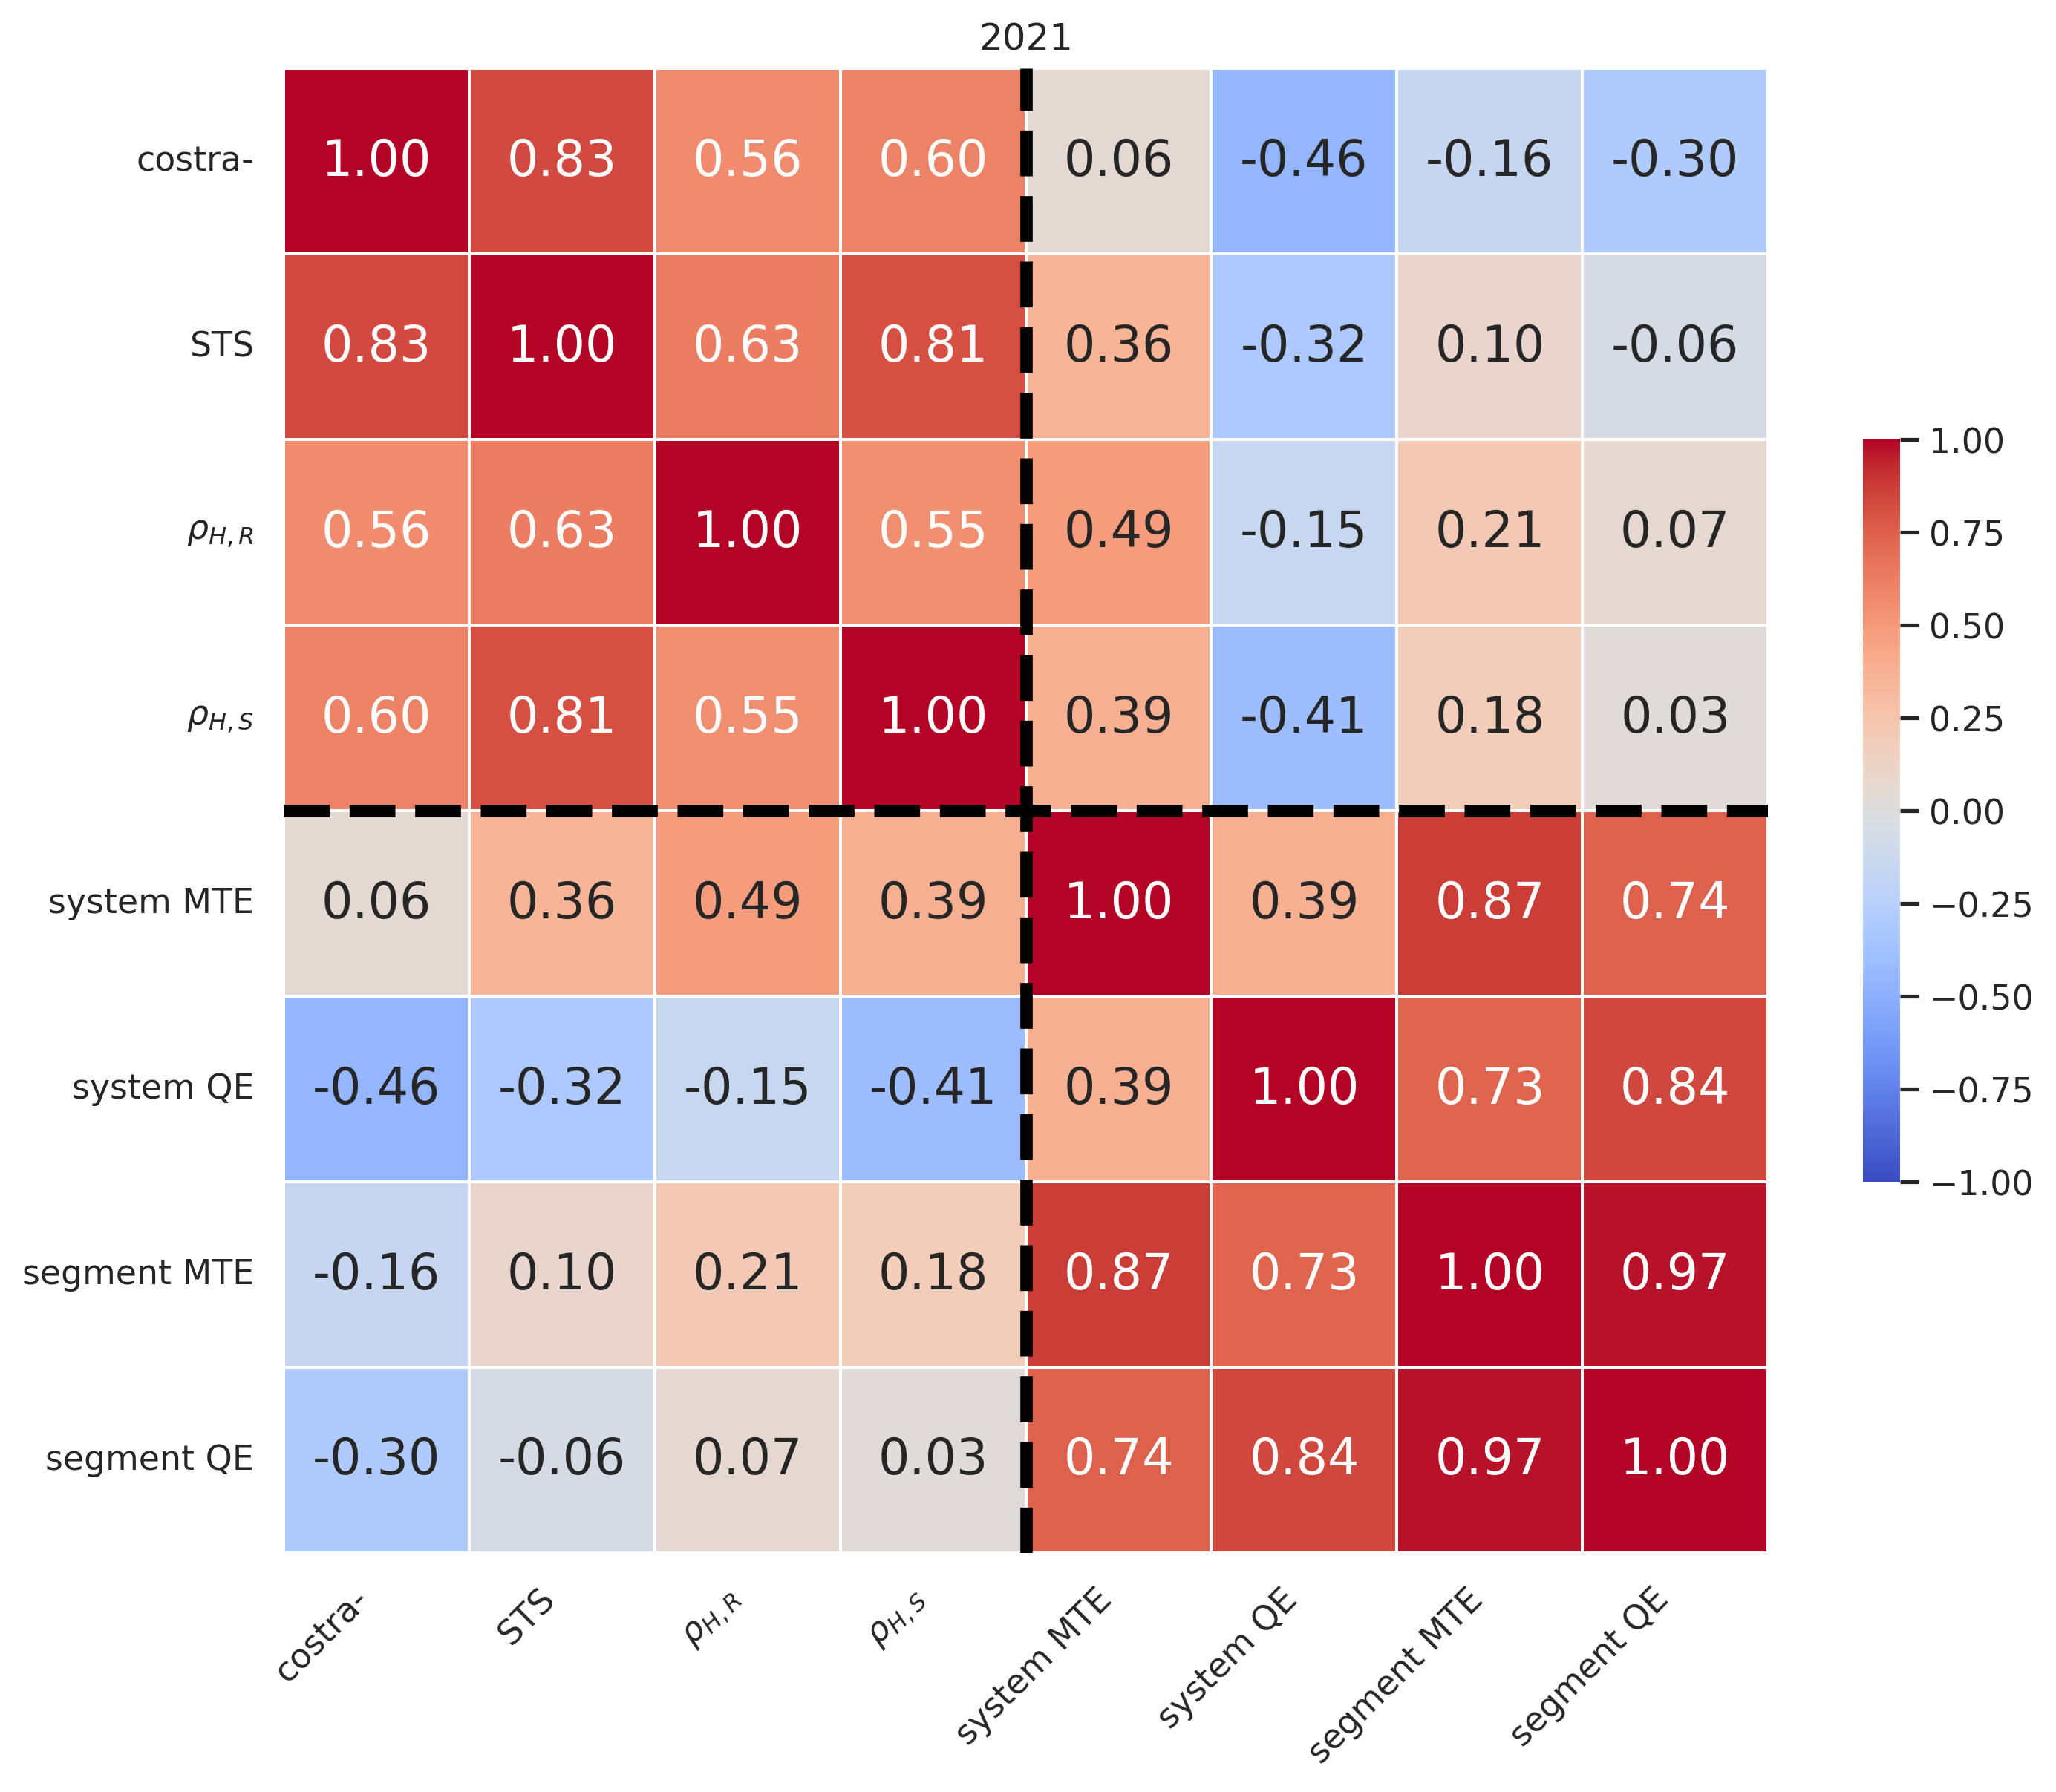
\includegraphics[width=0.8\linewidth]{correlation_heatmap_2021.png}
    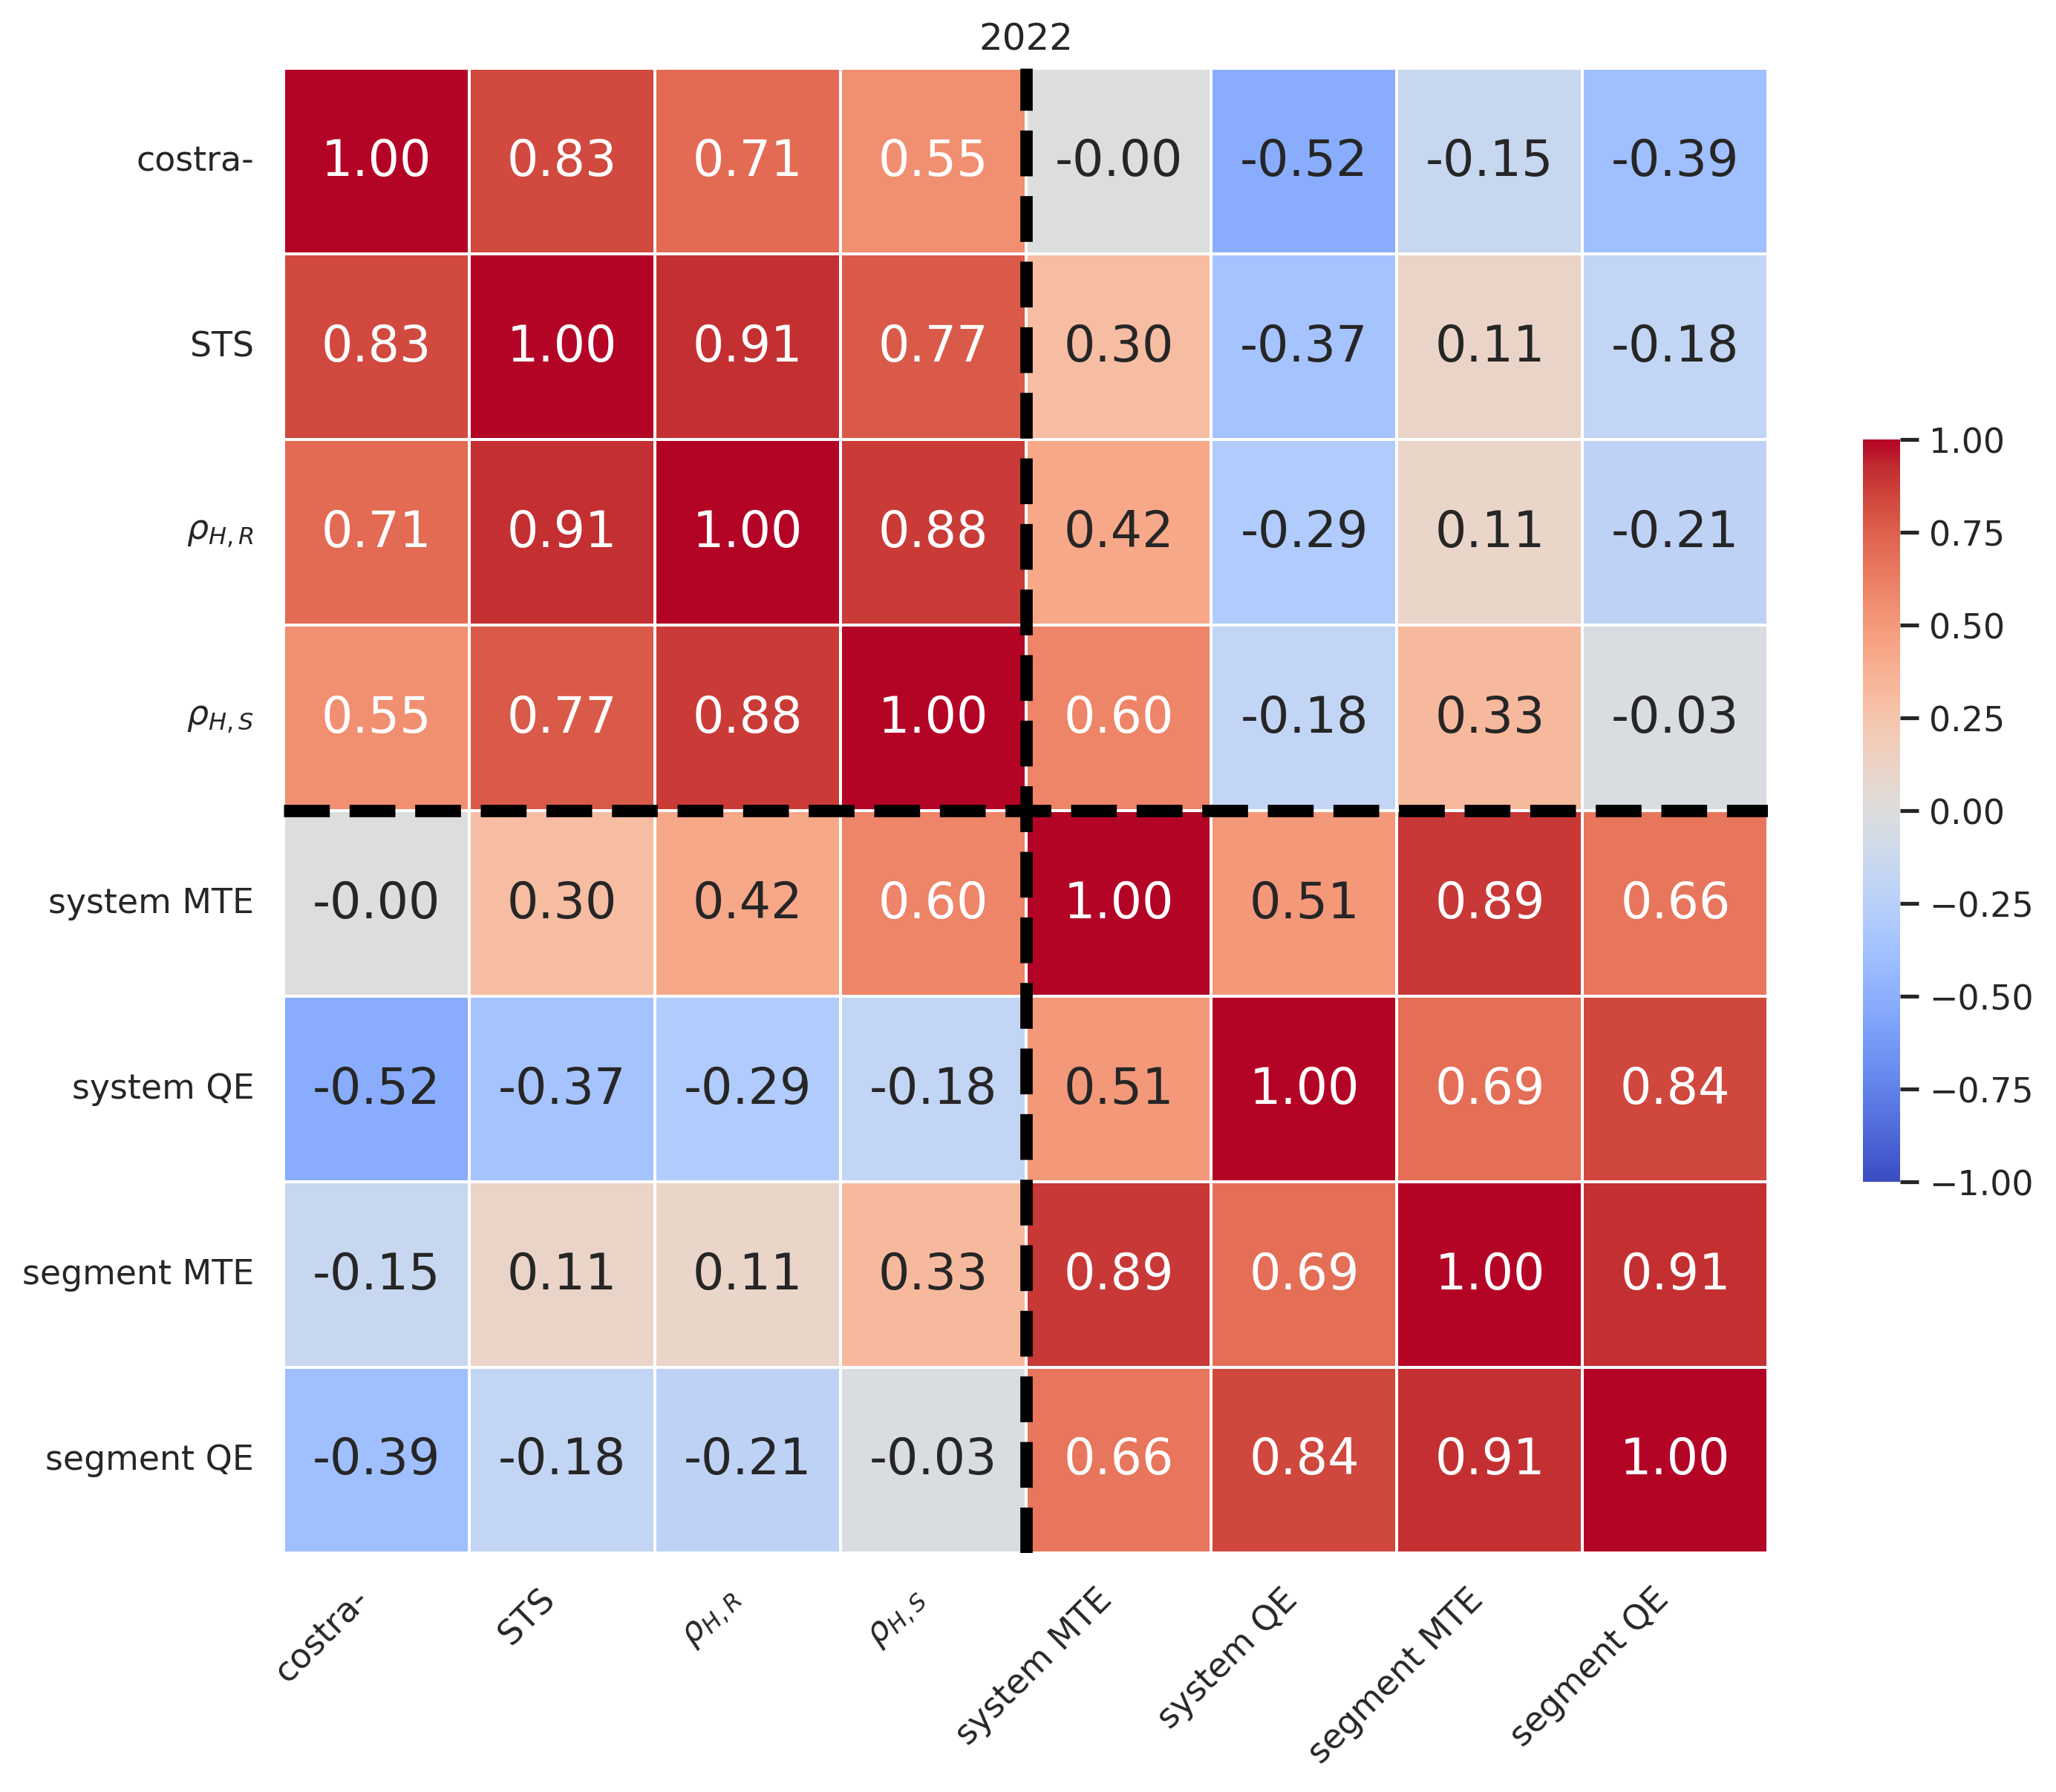
\includegraphics[width=0.8\linewidth]{correlation_heatmap_2022.png}
    \caption{Correlation heatmaps for different method of embedding evaluations. The heatmaps are intentionally kept in a rectangular shape to emphasize the mismatch in correlation patterns between intrinsic evaluation (\costraminus, STS, $\rho_{H,R}$, $\rho_{H,S}$) and extrinsic evaluation (system MTE/QE and segment MTE/QE).}
    \label{fig:heatmap}
\end{figure}

The correlation analysis between different evaluation methodologies, visualized by heatmaps in \Cref{fig:heatmap}, reveals interesting patterns of how different evaluation methodologies relate to each other. These patterns provide valuable insight into the reliability and consistency of various embedding evaluation approaches.

The heatmaps highlight a strong alignment among all intrinsic tasks (\costraminus, STS, and MTE baselines). Moreover, there is a strong correlation between the segment-level and the system-level metrics, indicating that aggregated segment scores provide reliable system-level insights. In particular, we observe strong correlations between segment-level metrics (\emph{segment MTE} and \emph{segment QE} showing correlations of 0.97 and 0.91 for 2021 and 2022 respectively), suggesting that these evaluation approaches capture similar aspects of translation quality despite their methodological differences.

%The relationship between reference-based and reference-free evaluation methods also presents interesting patterns. Although system-level MTE and QE show moderate positive correlation (0.39 in 2021, increasing to 0.51 in 2022), their segment-level counterparts demonstrate much stronger agreement (0.97 in 2021, 0.91 in 2022). This suggests that while these methods may diverge in system-level assessment, they tend to agree more strongly when evaluating individual translations.

However, one of the most striking findings is the weak and sometimes even negative correlation between intrinsic evaluation metrics \costraminus, STS) and the system-level quality estimation scores \emph{system QE}. This discrepancy is particularly evident in the 2022 data, where \costraminus shows a negative correlation (-0.52) with \emph{system QE}, challenging the assumption that better semantic representation capabilities necessarily translate to improved MT evaluation performance.

These findings suggest that intrinsic measures capture general semantic similarity, but do not fully reflect the aspects of meaning that are important for MTE or QE. In practice, this means that intrinsic benchmarks are not reliable for selecting embeddings for MT evaluation. Instead, our results point to the importance of fine-tuning and model capacity. At the same time, it remains unclear what properties an intrinsic evaluation would need to capture in order to be useful in this setting. One possible direction is to look more closely at the types of errors reflected in human MT evaluation, and to determine whether they are primarily semantic in nature or involve other aspects that current intrinsic benchmarks fail to represent.

\subsection{Conclusion}
We experimented with several evaluation methods for both Czech and multilingual sentence embeddings, considering intrinsic semantic tasks and downstream application in machine translation evaluation and quality estimation.

\begin{mdframed}[
    linecolor=gray,
    linewidth=2pt,
    roundcorner=5,
    backgroundcolor=gray!5
]
\noindent
We answered the following research questions:

\paragraph{Do intrinsic metrics (Costra, STS, baseline cosine) predict downstream MTE/QE performance?}
No, we observe a lack of correspondence between the two tasks for Czech data. Models that excel in STS/\costra (e.g., \simcse) do not translate into the best MTE/QE metrics after fine-tuning, while models with weak intrinsic scores (\xlmr, \hbox{\fernet{}}) become top performers once used within the \comet framework. The correlations between intrinsic scores (\costraminus, STS) and system-level QE are weak or negative, indicating that the tested intrinsic tasks are poor selectors for downstream MT evaluation.

% \XXX{ten FERNET, ktery vedl k tomu, ze radka zacinala zaviraci zavorkou, jsem zkusil zabalit to hboxu, to pomohlo. Jenom mit zaviraci zavorky za fernetem nestacilo. Asi je to ten xspace, ktery dela neplechu, fakt radsi nepouzivat a makra peclive ukoncovat slozenymi zavorkami{}.}
\paragraph{Are Czech-specific encoders better than multilingual embedders for evaluation of Czech translation in fine-tuned \comet metrics?}
Not decisively. There are no strong differences in performance between language-specific and multilingual models. Both categories are comparably represented among the top-performing models in intrinsic and extrinsic tasks.
% \item ?Zabrusovat do tohoto? Model architecture  seems more important than whether it's multilingual or monolingual
    
\paragraph{Does model size matter after fine-tuning for MTE/QE?}
Yes. In contrast to intrinsic tasks, fine-tuning embeddings for MTE/QE reveals that model size does matter, with the \Small embeddings consistently showing poor performance, while \Base/\LargeSize encoders provide richer representations that the regression head can leverage. 
   
\paragraph{Do references still provide clear benefits for the strongest models?}
Only marginally in our experiments. The top reference-based and reference-free estimators (\cometm{\fernet} vs. \cometq{\fernet}) achieve nearly identical correlations at both system and segment levels, suggesting a reduced marginal utility of references when encoders are strong. The same holds for the official ensemble baselines.

We also observed  stability of the correlations over time between the system-level \comet-based metrics, which provides encouraging evidence for the reliability of these evaluation approaches in contrast to traditional string-based metrics, which  remained competitive in 2021 but degraded substantially in 2022. 

\end{mdframed}
%\ml{Tohle je mov hezké Conclusion pro sekci  4.5 -- dalo by se něco podobného sepsat pro každou sérii experimentů? Líbí se mi ta forma - research questions a odpovědi!}

%These insights underscore the importance of aligning evaluation methodologies with downstream tasks and suggest that further research should explore refined intrinsic measures as well as the impact of architectural and size-related factors on model performance.

%Our experiments reveal an interesting disconnect: models that excel in intrinsic semantic similarity tests do not consistently yield superior performance on downstream translation evaluation tasks. Conversely, models with seemingly over-smoothed embedding spaces can, through fine-tuning, achieve excellent results. These findings highlight the complex relationship between semantic property probes and downstream task, emphasizing the need for more research into ``operationalizable semantics'' in sentence embeddings, or more in-depth downstream tasks datasets (here translation evaluation).